\section{Aufbau}
\label{sec:Aufbau}
\begin{figure}
	\centering
	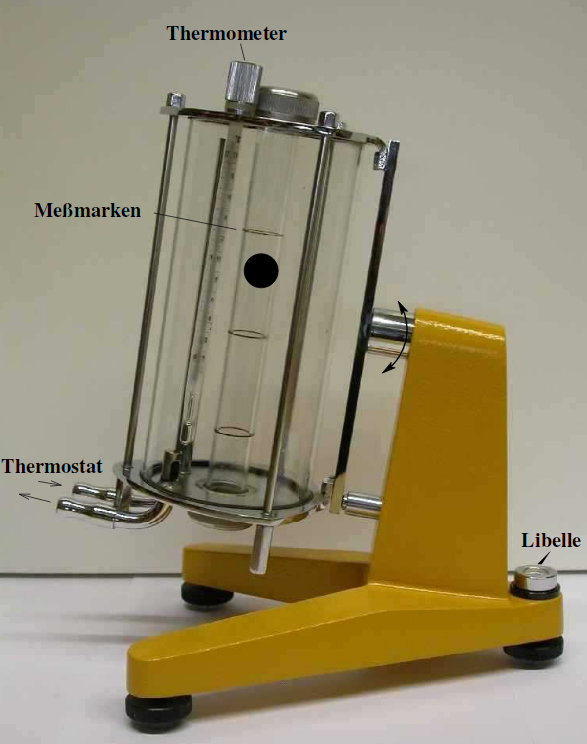
\includegraphics[width=\linewidth-100pt,height=\textheight-100pt,keepaspectratio]{content/Bilder/Hoeppler.png}
	\caption{Abbildung des Höppler-Viskosimeters \cite{V207}.}
	\label{fig:Aufbau2}
\end{figure}
Das Höppler-Viskosimeter besteht aus einer Glasröhre, welche mit der zu
untersuchenden Flüssigkeit gefüllt ist. In diese wird eine Kugel gesetzt, deren
Durchmesser nur geringfügig kleiner ist als der der Glasröhre. Damit die Kugel
nicht gegen die Wände der Fallröhre stößt, ist die Röhre leicht geneigt. Um ein bestimmtes Gefälle zu wahren
 kann das Viskosimeter über eine Libelle gerade ausgerichtet werden. Zur Messung
der Fallzeit sind Markierungen an der Röhre angebracht. Für eine erneute Zeitmessung
lässt sich das Viskosimeter an der Befestigung um $\SI{180}{\degree}$ drehen. Um die Temperaturabhängigkeit
der Viskosität zu untersuchen ist ein Wasserbad um die Fallröhre herum angebracht.
Diese kann über ein Thermostat kontrolliert erhitzt werden. Die Temperatur
kann über ein Thermometer überprüft werden. Dieses ist entweder am Thermostat oder 
direkt am Wasserbad angebracht.
